\section{Review of Polynomials (Optional)}
\label{sec.general}

%% By Geek3 - Own work, CC BY-SA 3.0, https://commons.wikimedia.org/w/index.php?curid=9552813
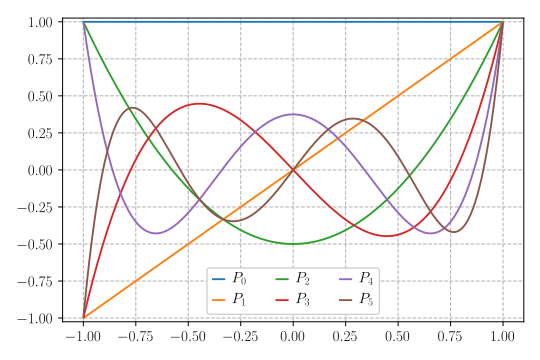
\includegraphics[width=0.9\textwidth]{Legendrepolynomials6.png}

Your goal in the next several sections is to find \emph{root} of
\emph{polynomials}.  This section (\S\ref{sec.general}) explains
the how and why the algorithm works.  The algorithm is summarized
in \S\ref{sec.algorithm} (page~\pageref{sec.algorithm})

If you want to start coding quickly, you skip directly to
\S\ref{sec.line} (page~\pageref{sec.line}).  If you are also
interested in the theory, you can quickly read over
\S\ref{sec.general}.


\subsection{What is a Polynomial?}

\begin{definition}{polynomial of degree n}{}
  A \emph{polynomial} of \emph{degree n} is a function of a single
  variable, usually $x$, of the form.
  \[P(x) = \alpha_n x^n + \alpha_{n-1} x^{n-1} + \cdots + \alpha_2 x^2 + \alpha_1 x + \alpha_0 \]

  where $\alpha_n, \alpha_{n-1}, \ldots, \alpha_0$ are called
  coefficients and may be integers, rational numbers, or real numbers.
\end{definition}

$P(x) = 2 x^4 + 5 x^3 + x^2 - x + 1$ is 4th degree polynomial.


Any of the coefficients after the leading one may be 0.  Terms with a coefficient of zero
are usually omitted.  $P(x) = 5 x^3 + x - 1$ is 3th degree polynomial
where the coefficient of the $x^2$ term is 0.


\subsection{Fundamental Theorem of Algebra}

\begin{definition}{root}{}
  If $P(x)$ is a polynomial, and $r$ is a number for which $P(r)=0$,
  then $r$ is called a \emph{root} of the polynomial.
\end{definition}

The polynomial $P(x) = x^3 - x$ as three roots, 1, -1, and 0.  We know
this because
\begin{align*}
  P(1) &= (1)^3 - 1 
  = 1 - 1 
  = 0\\[3pt]
  P(-1) &= (-1)^3 - (-1) 
  = -1 + 1 
  = 0\\[3pt]
  P(0) &= (0)^3 - 0
  = 0 - 0 
  = 0  
\end{align*}

The fact that $P(x) = x^3 - x$ has \emph{at least} three roots is easy
to verify simply by evaluating the function $P(x)$ at 1, -1, and 0.
Theorem~\ref{th.n.roots} claims something stricter; it claims that $P(x)$
has at most three roots.  But before getting to Theorem~\ref{th.n.roots}, we take a look at Theorem~\ref{th.ftoa}.


\begin{theorem}{Fundamental Theorem of Algebra}{ftoa}
  Every non-constant polynomial of degree~1 or higher has a root.
\end{theorem}

The Fundamental Theorem of Algebra claims that every polynomial has a root.
However, sometimes the root is complex.  For example the polynomial,
$P(x) = x^2 + 1$, has two (and only two) complex roots, where $i=\sqrt{-1}$.

\begin{align*}
  P(i) &= i^2 + 1 
  = -1 - 1 
  = 0\\[3pt]
  P(-i) &= (-i)^2 + 1 
  = (-1)^2(i)^2 + 1 = (1)(-1) + 1
  = 0
\end{align*}


From this point forward, in this atelier, we only
attempt to determine the real roots, ignoring the complex roots.  For
this reason, we will not be able to find all the roots of some
polynomials.

\begin{theorem}{Roots with Multiplicity}{n.roots}
  A polynomial of degree $n\ge 1$ has $n$ roots, some of which may be
  equal.
\end{theorem}
\begin{proof}

  [By Induction]
  
  \begin{itemize}
    
  \item \textbf{Base case:} If $n=1$, then Theorem~\ref{th.ftoa}
    guarantees it has a root; call it $r_1$.  Thus it is of the form
    $P(x)=\alpha (x-r_1)$.
  \item \textbf{Inductive case:} Suppose $n>1$.  Suppose every
    polynomial, $Q(x)$ of degree $n$ has $n$-many roots,
    $r_1,\ldots,r_n$, and can thus be written as:
    \[Q(x) = \alpha_1 (x - r_1) (x - r_2) \cdots (x - r_n)\]
    Now consider a polynomial, $P(x)$, of
    degree~$n+1$.  Theorem~\ref{th.ftoa} guarantees $P(x)$ has a root;
    call it $r_{n+1}$, thus $(x-r_{n+1})$ is a factor of $P(x)$ so there
    exists a polynomial, $Q(x)$, of degree~$n$ such that
    $P(x) =  Q(x) (x-r_{n_1})$.
    But by inductive hypothesis, $Q(x)$ can be written
    as \[Q(x) = \alpha_1 (x - r_1) (x - r_2) \cdots (x - r_n)\]
    So, \[P(x) = \alpha_1 (x - r_1) (x - r_2) \cdots (x - r_n) (x-r_{n+1})\]

    Thus $P(x)$ has $n+1$ roots.
  \end{itemize}
\end{proof}

\subsection{Algorithm for Finding Roots}
\label{sec.algorithm}

The proof of Theorem~\ref{th.n.roots} gives us the algorithm which we will use to find
roots in this atelier.  Given a degree~$n$ polynomial (for $2<n\leq5$),
\begin{enumerate}
\item If we successfully find a root, $r_n$ of the $n$-degree polynomial
\item Then we will factor  $(x-r_n)$ out of the polynomial,
\item Giving us new polynomial but with degree~$n-1$,
\item Which we can solve by the same approach.  
\item This process continues until we reach degree~$n=2$ which we
  solve using the quadratic formula.

\end{enumerate}


% LocalWords:  atelier
